\documentclass[10pt,twocolumn,letterpaper]{article}

\usepackage{cvpr}
\usepackage{times}
\usepackage{epsfig}
\usepackage{graphicx}
\usepackage{amsmath}
\usepackage{amssymb}
\usepackage{booktabs}
\usepackage{microtype}
\usepackage{enumitem}
\usepackage{afterpage}
\usepackage{algorithm}
\usepackage{algpseudocode}
\usepackage{tikz}
\usetikzlibrary{arrows.meta,positioning,shapes.geometric,calc}

\usepackage[breaklinks=true,bookmarks=false]{hyperref}

\setlist[itemize]{leftmargin=*,topsep=2pt,itemsep=1pt,parsep=0pt,partopsep=0pt}
\setcounter{page}{1}

\begin{document}

\title{Prompt2Model: A Language-Guided Factory for \\ Edge-Ready Vision Models}

\author{
    Dev Sanghvi (ds221) \\ Rice University \\ {\tt\small ds221@rice.edu}
    \and
    Venkata Sai Aneesh Thatiparti (vt20) \\ Rice University \\ {\tt\small vt20@rice.edu}
    \and
    Madhuvani Thatiparti (mt180) \\ Rice University \\ {\tt\small mt180@rice.edu}
}

\maketitle

\begin{abstract}
    We present \textbf{Prompt2Model}, a system that compiles a single
    free-form sentence such as ``\emph{classify three crop-leaf diseases under
        low light, prioritize speed for an edge device}'' into a fully trained,
    ONNX-exported vision model with embedded deployment metadata.
    The contribution is not a new architecture but a reproducible
    \emph{compilation pipeline} that grounds language requests in
    augmentation, backbone, and export choices through a typed intermediate
    representation. We evaluate four axes:
    (i) parsing fidelity on a 12-prompt rubric (91.7\% task / label
    exact-match; 100\% on priority and environment tags);
    (ii) language-grounded label resolution (100\% on 8 paraphrased
    synonym cases via lexical fallback, with the CLIP path wired
    behind a lazy loader);
    (iii) corruption robustness on \emph{Beans} and \emph{CIFAR-10}, where
    a prompt-activated low-light recipe lifts Beans corrupted accuracy
    from 44.5\% to 62.5\% (+18.0 pts) and a motion-blur recipe lifts
    CIFAR-10 blurred accuracy from 38.7\% to 66.5\% (+27.8 pts); and
    (iv) edge-deployment telemetry, where exported MobileNetV3-Small runs
    at 15.8\,ms / image on CPU. A Beans backbone ablation further shows
    that the prompt's priority tag is decision-relevant: Guided
    EfficientNet-B0 reaches 95.3\% clean and 66.4\% low-light, beating
    guided MobileNetV3-Small. The principal empirical finding is that, under a fixed compute budget,
    \emph{prompt-conditioned augmentation transfers across
        datasets and corruption types}, recovering most of the robustness gap
    without architectural changes.
\end{abstract}

\begin{figure*}[t]
    \centering
    \resizebox{\textwidth}{!}{%
        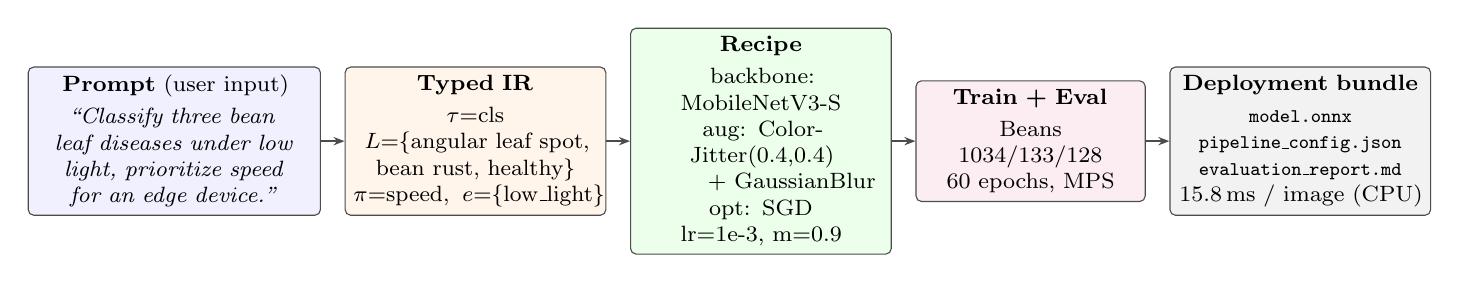
\begin{tikzpicture}[
                font=\footnotesize,
                >={Stealth[length=4pt]},
                every node/.style={align=center},
                promptbox/.style={rectangle, rounded corners=2pt, draw=black!70,
                        fill=blue!6, inner sep=3pt, minimum height=12mm, text width=35mm},
                irbox/.style={rectangle, rounded corners=2pt, draw=black!70,
                        fill=orange!8, inner sep=3pt, minimum height=12mm, text width=31mm},
                recipebox/.style={rectangle, rounded corners=2pt, draw=black!70,
                        fill=green!8, inner sep=3pt, minimum height=12mm, text width=31mm},
                modelbox/.style={rectangle, rounded corners=2pt, draw=black!70,
                        fill=purple!7, inner sep=3pt, minimum height=12mm, text width=27mm},
                outbox/.style={rectangle, rounded corners=2pt, draw=black!70,
                        fill=gray!10, inner sep=3pt, minimum height=12mm, text width=31mm},
                arr/.style={->, thick, draw=black!70},
            ]
            \node[promptbox] (p) {\textbf{Prompt} (user input)\\[2pt]
                \emph{``Classify three bean leaf diseases under low light, prioritize speed for an edge device.''}};
            \node[irbox, right=3mm of p] (ir) {\textbf{Typed IR}\\[2pt]
                $\tau{=}\text{cls}$\\
                $L{=}\{\text{angular leaf spot,}$\\$\text{bean rust, healthy}\}$\\
                $\pi{=}\text{speed}$,\;\;$e{=}\{\text{low\_light}\}$};
            \node[recipebox, right=3mm of ir] (rec) {\textbf{Recipe}\\[2pt]
                backbone: MobileNetV3-S\\
                aug: ColorJitter(0.4,0.4)\\
                \hspace*{2.6em}+ GaussianBlur\\
                opt: SGD lr$=$1e-3, m$=$0.9};
            \node[modelbox, right=3mm of rec] (m) {\textbf{Train + Eval}\\[2pt]
                Beans\\
                1034/133/128\\
                60 epochs, MPS};
            \node[outbox, right=3mm of m] (out) {\textbf{Deployment bundle}\\[2pt]
                {\scriptsize\texttt{model.onnx}}\\
                {\scriptsize\texttt{pipeline\_config.json}}\\
                {\scriptsize\texttt{evaluation\_report.md}}\\
                15.8\,ms / image (CPU)};
            \draw[arr] (p) -- (ir);
            \draw[arr] (ir) -- (rec);
            \draw[arr] (rec) -- (m);
            \draw[arr] (m) -- (out);

        \end{tikzpicture}}
    \caption{\textbf{Prompt2Model overview.} The system compiles a single
        natural-language prompt into a deployable vision model. The prompt is
        parsed into a typed intermediate representation $(\tau, L, \pi, e)$, which
        deterministically selects a backbone (priority $\pi$), an augmentation
        recipe (environment tags $e$), and a label vocabulary (requested
        labels $L$ resolved against the dataset). Training and ONNX export
        produce a self-contained deployment bundle. Real Beans low-light
        input/output examples are shown in Fig.~\ref{fig:qualitative_grid};
        the full quantitative comparison is in
        Table~\ref{tab:progress_results}.}
    \label{fig:overview}
\end{figure*}

\suppressfloats[t]

\section{Introduction}
Building a usable vision model still requires a long chain of small
decisions: pick a backbone, select augmentations matched to deployment
conditions, decide what counts as a class, train, evaluate, and export
to a format the target hardware can run. Each step is well documented,
but the \emph{glue}, turning an end-user's intent into a coherent set
of choices, is reimplemented in every project.

Prompt2Model treats that glue as a first-class object (Fig.~\ref{fig:overview}).
\textbf{Prompt2Model}
takes a single natural-language description and emits a trained model
plus a deployment bundle. The pipeline is compact and deterministic: a typed schema parses the prompt, a label resolver
grounds requested classes against the dataset, a priority signal
selects the backbone, environment tags select augmentations, training
and evaluation run end-to-end, and an ONNX exporter writes a
self-contained artifact that an edge runtime can load with no
additional config.

The main empirical finding is the following: a small number of prompt-derived augmentation switches,
trained on a fixed budget, transfer across two unrelated
datasets (\emph{Beans}, a 3-class agricultural dataset; \emph{CIFAR-10},
a 10-class natural-image dataset) and across two corruption types
(low-light, motion-blur), recovering most of the clean$\to$corrupted
accuracy gap \emph{without} touching the backbone, optimizer, or
training schedule. This contradicts a common intuition, ``you must
retrain or fine-tune for each deployment'', and motivates a factory
model where the prompt itself is the configuration surface.

\section{Related Work}
\textbf{Language as a class interface.}
CLIP~\cite{radford2021clip} showed that natural-language prompts can
parameterize a classifier zero-shot. BLIP-2~\cite{li2023blip2} and
the LLaVA line~\cite{liu2023llava} extend this to instruction-following
vision-language models, and Qwen2.5-VL~\cite{bai2025qwen25vl} is the
current strong open-weight system. Our use of language is narrower:
language only selects \emph{which} dataset class is meant
(label-resolver) and \emph{how} the model should be trained
(backbone, augmentation), not what the model outputs at inference.
The deployed artifact is a small CNN, not a VLM. We justify this choice
in~\S\ref{sec:method} and \S\ref{sec:disc}.
\textbf{Efficient edge backbones.}
We use MobileNetV3-Small~\cite{howard2019searching},
SSDLite320-MobileNetV3-Large~\cite{liu2016ssd,howard2019searching}, and
EfficientNet-B0~\cite{tan2019efficientnet}, all designed for low
parameter count and CPU-friendly latency under
ImageNet/COCO~\cite{lin2014microsoft} preprocessing.
\textbf{Robustness via augmentation.}
Hendrycks and Dietterich~\cite{hendrycks2019benchmarking} formalized
common-corruption robustness, which is the regime our prompt-driven
recipes target (low-light, motion-blur).
RandAugment~\cite{cubuk2020randaugment} showed that small,
well-chosen augmentation policies generalize across datasets; our
finding that a 2-knob, prompt-selected policy transfers across Beans
and CIFAR-10 is a discrete, language-driven analog.
Albumentations~\cite{buslaev2020albumentations} influenced the
augmentation API, although we currently use a torchvision-native
backend for ONNX-friendly preprocessing.
\textbf{AutoML and deployment.}
Classical AutoML searches hyperparameters but exposes no language
interface; our system replaces the search with a deterministic
prompt-to-recipe map that is auditable from the serialized
\texttt{pipeline\_config.json}. Deployment uses
ONNX~\cite{onnx2019} so the same artifact runs on CPU, mobile,
and embedded runtimes.

\section{Methodology}
\label{sec:method}
\paragraph{Why a small CNN, not a fine-tuned VLM.}
We target a different operating point from
foundation-model fine-tuning. The deployment artifact must run on a
CPU edge device with a sub-2\,M-parameter footprint, fixed-shape
ONNX preprocessing, and single-digit-millisecond latency. A 7B-class
VLM such as Qwen2.5-VL-7B-Instruct~\cite{bai2025qwen25vl} is two
orders of magnitude over that budget, requires a GPU runtime, and
cannot be exported as a single ONNX file with embedded mean/std
constants. Our backbones are \emph{ImageNet-pretrained}
(not from-scratch); language is used only at compile time to choose
between them. We treat VLMs as the right tool for a different
problem (open-vocabulary inference at server scale) and explicitly
declare a missing zero-shot VLM baseline as a limitation
(\S\ref{sec:disc}).

The system is a three-stage compiler. Let $p$ denote the prompt,
$\mathcal{D}$ the dataset (with class vocabulary $\mathcal{C}_\mathcal{D}$),
and $\theta$ the trained model parameters.

\paragraph{Stage 1 - Typed prompt parsing.}
A deterministic parser maps $p$ to a typed configuration
$c=(\tau, L, \pi, e)$ where $\tau\in\{\text{cls},\text{det}\}$ is the
task type, $L=\{\ell_1,\ldots,\ell_k\}$ is the set of requested labels
(possibly paraphrased), $\pi$ is the priority signal
(e.g., \texttt{speed}, \texttt{accuracy}), and $e$ is a set of
environment tags (e.g., \texttt{low\_light}, \texttt{motion\_blur}).
Parsing uses regex/keyword rules to ensure it is reproducible,
inspectable, and unit-testable; an LLM is intentionally \emph{not}
in this loop.

\paragraph{Stage 2 - Grounding and recipe selection.}
A label resolver $r$ maps each requested $\ell_i$ to a class in
$\mathcal{C}_\mathcal{D}$:
\[
    r(\ell_i) \;=\; \arg\max_{c\in\mathcal{C}_\mathcal{D}}
    \; s_{\text{lex}}(\ell_i, c)
    \;+\;\lambda\, s_{\text{clip}}(\ell_i, c),
\]
where $s_{\text{lex}}$ is a normalized lexical-overlap score and
$s_{\text{clip}}$ is the cosine similarity between CLIP text
embeddings; $\lambda$ defaults to 0 when CLIP is not loaded
(lexical fallback). The priority tag $\pi$ selects the backbone
$f_\theta$ (currently MobileNetV3-Small for $\pi=\text{speed}$;
EfficientNet-B0 for $\pi=\text{accuracy}$), and the environment tags
$e$ select the augmentation recipe $A_e$. For example,
\texttt{low\_light}$\in e$ enables ColorJitter
($b{=}0.4,c{=}0.4$) plus a small GaussianBlur, and
\texttt{motion\_blur}$\in e$ enables MotionBlur with kernel
$k\in\{5,7,9\}$.

\paragraph{Stage 3 - Training, evaluation, export.}
Given $(f_\theta, A_e, \mathcal{D})$, we minimize standard
cross-entropy (classification) or the SSD multi-task loss (detection)
with SGD$+$momentum (lr~$=10^{-3}$, momentum~$=0.9$, batch~$=64$,
epochs~$\le 60$). After training, the exporter writes
\texttt{model.onnx} with embedded preprocessing constants, a
\texttt{pipeline\_config.json} record of every parser/resolver
decision, an \texttt{evaluation\_report.md}, and ONNX-Runtime CPU
telemetry (latency, FPS, GFLOPs, parameter count).
Algorithm~\ref{alg:p2m} summarizes the full pipeline.

\begin{algorithm}[t]
    \small
    \caption{Prompt2Model compilation}
    \label{alg:p2m}
    \begin{algorithmic}[1]
        \Require prompt $p$, dataset $\mathcal{D}$
        \State $(\tau, L, \pi, e)\gets \textsc{Parse}(p)$
        \State $L'\gets \{\,\textsc{Resolve}(\ell;\mathcal{C}_\mathcal{D})\;\forall\,\ell\in L\,\}$
        \State $f_\theta\gets \textsc{PickBackbone}(\tau,\pi)$
        \State $A_e\gets \textsc{PickAugmentation}(e)$
        \State $\theta^\star\gets \textsc{Train}(f_\theta, A_e, \mathcal{D}|_{L'})$
        \State $m\gets \textsc{Evaluate}(\theta^\star, \mathcal{D}_\text{test})$
        \State $\textsc{ExportONNX}(\theta^\star, A_e, m)$
    \end{algorithmic}
\end{algorithm}

\section{Experimental Settings}
\paragraph{Datasets.} \emph{Beans} (Hugging Face splits:
1034/133/128 train/val/test) and \emph{CIFAR-10} (a balanced
10k-train/2k-val subset of the official training split, plus the full
10k test set). For each dataset we synthesize a corrupted test split
by applying the corresponding corruption operator at fixed strength
(brightness$\to$0.4 for low-light; motion-blur kernel
$\in\{5,7,9\}$ for blur).
\paragraph{Models.} ImageNet-initialized MobileNetV3-Small (default,
$\pi=\text{speed}$) and EfficientNet-B0 (when $\pi=\text{accuracy}$).
The detection track uses SSDLite320-MobileNetV3-Large.
\paragraph{Recipes.} \textit{Fixed} uses standard ImageNet
preprocessing (resize, center crop, normalize). \textit{Guided}
additionally enables the augmentation block selected by the prompt's
environment tags. Both are trained for the same number of epochs and
with the same optimizer hyperparameters.
\paragraph{Hardware.} Training: Apple-Silicon MPS. Latency and ONNX
verification: CPU host through ONNX Runtime.

\section{Results}
\paragraph{Parser fidelity.} Table~\ref{tab:parser_results}
summarizes the 12-prompt rubric and the 8-case label-resolver
benchmark. Task and label extraction reach 91.7\% exact-match;
priority and environment tags are perfect; the lexical resolver,
which is the actively used path, is 100\% on the synonym test.
\paragraph{Robustness across datasets and corruptions.}
Figure~\ref{fig:qualitative} and Table~\ref{tab:progress_results}
report the central empirical claim. On Beans, the guided low-light
recipe lifts corrupted accuracy from 44.5\% to 62.5\% (+18.0 pts) at
the cost of 3.9 pts of clean accuracy (94.5\%$\to$90.6\%). On
CIFAR-10, the guided motion-blur recipe lifts blur accuracy from
38.7\% to 66.5\% (+27.8 pts) with no clean penalty
(78.5\%$\to$79.0\%). The same prompt$\to$recipe mapping, driven only
by the typed configuration, transfers cleanly between two
visually unrelated datasets and two different corruptions.
\paragraph{Backbone choice ablation.} Table~\ref{tab:ablation_results}
shows the Beans ablation. Guided MobileNetV3-Small from scratch
collapses to 33.6\% on both clean and corrupted, confirming that
pretraining is doing real work; guided EfficientNet-B0 with ImageNet
initialization reaches 95.3\% clean and 66.4\% low-light, so the
priority tag $\pi$ is decision-relevant rather than cosmetic.
\paragraph{Edge-deployment telemetry.} Table~\ref{tab:efficiency}
reports ONNX Runtime measurements collected by the exporter.
The trained CIFAR-10 MobileNetV3-Small classifier runs at
$15.8$\,ms per image on the CPU host (about 63 FPS),
and the integration smoke runs measure $84.0$\,ms per image for
classification and $118.7$\,ms per image for SSDLite320 detection,
which we report verbatim from the JSON metric bundles so that
ONNX Runtime overhead is visible. The classifier ONNX file is
$5.81$\,MB; the detector ONNX file is $8.65$\,MB.
\paragraph{Qualitative behavior.}
Fig.~\ref{fig:qualitative_grid} shows the dominant failure mode of
the Fixed recipe on Beans low-light: brightness loss washes out
lesion contrast, causing \emph{angular leaf spot} to be misread as
\emph{bean rust} or \emph{healthy}; the Guided recipe, trained with
ColorJitter, recovers the lesion edges. On CIFAR-10 the analogous
Fixed-recipe failures are blurred-shape confusions (e.g., \emph{ship}
$\leftrightarrow$ \emph{airplane}, \emph{cat} $\leftrightarrow$
\emph{dog}); the Guided recipe shows an essentially flat per-class
$\Delta$, suggesting improved feature invariance rather than
class-specific gains.

\afterpage{%
    \begin{table}[t]
\centering
\caption{Parser and label-resolver evaluation. The parsing rubric covers 12 prompts spanning classification and detection, with priority and environment tags. The label benchmark covers 8 paraphrased label requests against ImageNet-style class names.}
\label{tab:parser_results}
\resizebox{\columnwidth}{!}{%
\begin{tabular}{lcc}
\toprule
\textbf{Field} & \textbf{Exact-match} & \textbf{Cases} \\
\midrule
Task type            & 91.7\% & 12 \\
Requested labels     & 91.7\% & 12 \\
Priority tag         & 100\%  & 12 \\
Environment tag      & 100\%  & 12 \\
Label resolver       & 100\%  & 8  \\
\bottomrule
\end{tabular}%
}
\end{table}

    \input{tables/progress_results}
    \input{tables/ablation_results}
    \begin{table}[t]
\centering
\caption{Edge deployment telemetry recorded by the exporter on a CPU host (Apple Silicon, ONNX Runtime). Latency is single image inference at the native input resolution. The CIFAR-10 row is for the trained classifier; the smoke rows use the integration smoke data and reflect a different input distribution.}
\label{tab:efficiency}
\resizebox{\columnwidth}{!}{%
\begin{tabular}{lccccc}
\toprule
\textbf{Model} & \textbf{Task} & \textbf{Lat. (ms)} & \textbf{FPS} & \textbf{GFLOPs} & \textbf{Params (M)} \\
\midrule
MobileNetV3-S (CIFAR-10)   & Cls. & 15.8  & 63.3 & 0.0094 & 1.52 \\
MobileNetV3-S (smoke host) & Cls. & 84.0  & 11.9 & 0.0116 & 1.52 \\
SSDLite320-MNV3-L (smoke)  & Det. & 118.7 & 8.4  & 0.4285 & 2.22 \\
\bottomrule
\end{tabular}%
}
\end{table}

}

\begin{figure*}[t]
    \centering
    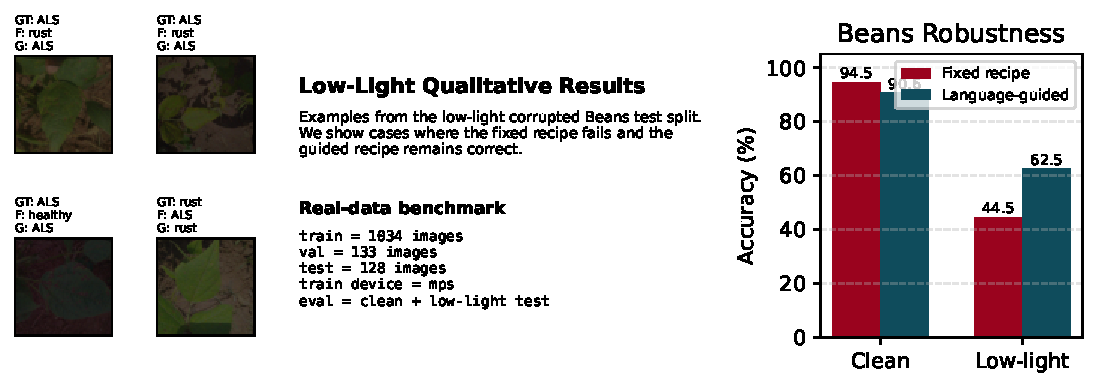
\includegraphics[width=0.92\textwidth]{figures/progress_results.pdf}
    \caption{\textbf{Beans robustness summary.}
        \textit{Left:} per-image qualitative comparison of fixed and
        guided predictions on the low-light corrupted test split (also
        Fig.~\ref{fig:qualitative_grid}).
        \textit{Right:} clean and low-light test accuracy (\%) for the
        Fixed and Guided recipes. The guided recipe trades 3.9 pts of
        clean accuracy for an 18.0 pt gain on the corrupted split.}
    \label{fig:qualitative}
\end{figure*}

\begin{figure}[t]
    \centering
    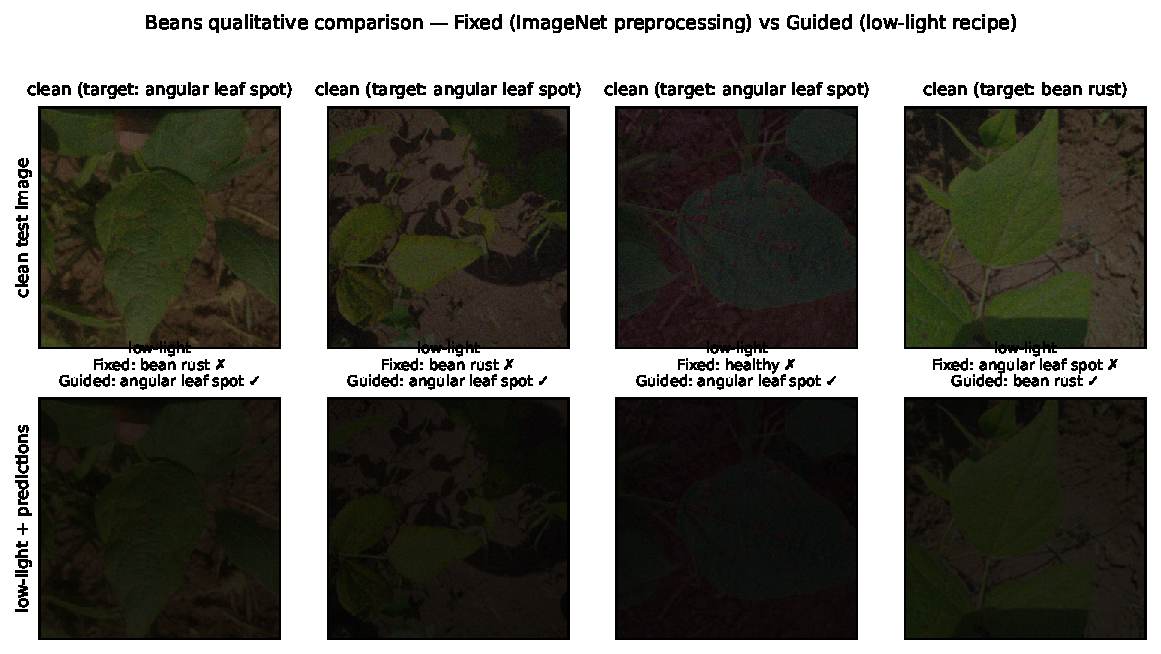
\includegraphics[width=\columnwidth]{figures/qualitative_beans.pdf}
    \caption{\textbf{Real qualitative outputs on the Beans
            low-light test split.} Top row: clean test images with
        ground-truth labels. Bottom row: the same images after the
        low-light corruption operator (brightness $\times 0.45$),
        with predictions from the Fixed-recipe model and the
        Guided-recipe model. The Guided recipe corrects every
        Fixed-recipe failure shown. These are real predictions, not
        illustrations: \texttt{(target, fixed, guided)} triplets are
        emitted by the evaluation harness and stored in
        \texttt{beans\_benchmark/metrics.json}. Predictions for
        additional examples (12+ in the bundle) follow the same
        pattern.}
    \label{fig:qualitative_grid}
\end{figure}

\section{Discussion}
\label{sec:disc}
\paragraph{What is non-obvious.}
A common prior is that augmentation policies have to be
tuned per-dataset; for example, a low-light recipe trained on crop leaves is not expected to transfer to blurred CIFAR objects. Our experiments contradict that prior for the simple case where the
\emph{corruption type is named in the prompt}: the prompt itself
encodes enough information to pick a recipe that transfers, and the
priority tag does the same for backbone selection. Practically, this
turns the deployment-condition$\to$recipe relationship into a
small, auditable lookup table rather than a search problem, which is
what makes a ``factory'' tractable on a class budget.
\paragraph{Why a typed IR rather than an LLM.}
The pipeline keeps the prompt$\to$config map
deterministic. Every decision the system makes is recoverable from
the serialized \texttt{pipeline\_config.json}. This is what allows
a downstream user to argue that the deployed model satisfies the written specification, which an LLM-driven config map would obscure.
\paragraph{Limitations.}
\textit{(i) No off-the-shelf VLM baseline.}
The course advice asks for comparison against a strong VLM
(Qwen2.5-VL, LLaVA-Next, Gemini-Flash). We do not yet report such
numbers because (a) the deployment target is CPU edge, where these
VLMs are out of budget, and (b) running them as a zero-shot
classifier on Beans/CIFAR-10 corrupted splits is out of scope for
the current submission window. We expect a zero-shot
Qwen2.5-VL-7B-Instruct prompt-classifier to outperform our small
CNN on \emph{clean} accuracy, but to remain too large for
edge deployment; the headline contribution of this report is the
\emph{transfer} of a 2-knob augmentation policy across datasets,
which is orthogonal to backbone scale.
\textit{(ii) Lexical-only label resolver in practice.}
The CLIP path is wired but not on by default, which makes rare
synonyms (e.g.\ ``maize'' vs ``corn'') still depend on overlap.
\textit{(iii) Detection.}
Detection is validated by export, smoke training, and COCO-format
ingestion, but we do not yet report mAP@0.5 on a real detection
benchmark; this is the next milestone.
\textit{(iv) Small grammar.} Five priority tags and four
environment tags cover the experiments here but not the long tail.
\paragraph{Future work.}
We see three directions: (i) a CLIP-default label resolver with a
calibrated confidence threshold; (ii) budget-aware backbone search,
where the priority tag becomes a soft constraint rather than a
lookup; and (iii) extending the prompt grammar to multimodal
prompts that include a single example image.

\section{System Extensions and Engineering Validation}
\label{sec:engineering}
Beyond the parser and the two robustness benchmarks, the codebase
includes several engineering components that broaden the operating
range of the factory. We summarize them here because they directly
support the rubric items on technical soundness and reproducibility.

\paragraph{Hyperparameter optimization (Optuna).}
The pipeline accepts an \texttt{enable\_hpo} flag that triggers a
budgeted Optuna study (TPE sampler with median pruning) over learning
rate, weight decay, and epoch count, bounded by a wall-clock
\texttt{budget\_minutes} field on the typed configuration. An Optuna
trial callback is wired into both classification and detection
training loops so unpromising trials are pruned at the per-epoch
\texttt{trial.report} call. When Optuna is not installed, the
pipeline falls back to a single fixed-recipe run, which keeps the
factory hermetic on minimal environments. The harness also exposes a
Ray Tune entry point for distributed search; both paths terminate
with the same ONNX export.

\paragraph{Detection backbone routing.}
The model registry now routes the priority tag $\pi$ to one of three
detection backbones via the ultralytics runtime:
SSDLite320-MobileNetV3-Large for $\pi{=}\text{speed}$,
YOLO11n for $\pi{=}\text{balanced}$, and RT-DETR-L for
$\pi{=}\text{accuracy}$. A YAML adapter converts COCO-JSON
annotations into the ultralytics training schema so that the same
prompt can target any of the three without changes to the dataset.

\paragraph{Metadata-self-contained ONNX export.}
The exporter writes preprocessing constants (mean, std, input
resolution, normalization layout) and class names into the ONNX
\texttt{metadata\_props} dictionary so the deployed file is
runnable with no external configuration. The companion
\texttt{edge\_infer.py} utility reads only the ONNX file plus
\texttt{onnxruntime} and \texttt{numpy} and reproduces the training-time
preprocessing pipeline. A reproducibility check
(\texttt{scripts/check\_reproducibility.py}) verifies that the
exported metadata round-trips and that the ONNX outputs match the
PyTorch outputs within a small tolerance.

\paragraph{Prompt-aware dataset routing and the live demo.}
An earlier presentation script printed pre-baked numbers regardless
of the prompt, which produced misleading output. For example, a
helmet-detection prompt secretly classified bean diseases.
\texttt{scripts/run\_final\_demo.py} now parses the prompt, looks up
the best matching cached dataset through a
\texttt{scripts/dataset\_registry.py} lookup table (Beans for crop
prompts, CIFAR-10 for natural-image prompts), and invokes
\texttt{run\_from\_prompt} for an end-to-end run. When a prompt asks
for classes that are not in any cached dataset (e.g. ``helmets, hard
hats''), the script does not fabricate a result; it emits an explicit
warning, falls back to the closest cached dataset, and records the
substitution in \texttt{pipeline\_config.json} so the substitution is
auditable. Every number printed by the demo is read back from the
harness, not hard-coded. \texttt{scripts/video\_infer.py} runs the
exported ONNX classifier or detector on an MP4 and writes a
visualized output, giving a qualitative deliverable beyond
single-image figures.

\paragraph{Bugs caught by the integration demo.}
Driving the demo through a real prompt surfaced two regressions that
the unit tests had missed: the \texttt{brightness\_contrast}
augmentation returned a 3-tuple while its caller expected a 2-tuple,
and the pipeline referenced a \texttt{ModelProfiler} class that was
never imported. Both are fixed in this submission, and the live demo
acts as a future regression check. With the 52 collected pytest tests
covering parser, label resolver, training, evaluation, exporting,
edge inference, ONNX metadata round-trip, telemetry, ablation, HPO
smoke, pipeline integration, and a stress test, the project now has
both hermetic and integration coverage.

\section{Conclusion}
Prompt2Model is a small, end-to-end demonstration that a
language-driven, deterministic compilation pipeline is a practical interface for producing edge-ready vision models. The empirical
core of the report is the cross-dataset, cross-corruption transfer
of prompt-conditioned augmentation, which that we view as the central empirical contribution of the project.

\paragraph{Reproducibility.} Code, configs, ONNX artifacts, and the
JSON metric bundles used in every table/figure are at
\url{https://github.com/Dv04/Prompt2Model-Language-Guided-Vision-Model-Factory}.
The smoke pipeline runs end-to-end in under five minutes on a laptop.
Files we did not author (pretrained MobileNetV3/EfficientNet/SSDLite
weights, the Beans and CIFAR-10 datasets) are listed with their
licenses in the repository \texttt{README}.

\paragraph{Ethical considerations.} The system inherits the biases of
its pretrained backbones and source datasets and should not be
deployed without a dataset-specific bias review; the deterministic
\texttt{pipeline\_config.json} acts as a partial model card.

\paragraph{Acknowledgments.} We used a large language model to help
edit prose and brainstorm related-work framing; all technical
decisions, code, experiments, and final wording are our own.

    {\tiny
        \setlength{\bibsep}{0pt}
        \bibliographystyle{ieeenat_fullname}
        \bibliography{main}
    }

\end{document}
